\documentclass{article}

\usepackage[final]{neurips_2024}

\usepackage[utf8]{inputenc}
\usepackage[T1]{fontenc}
\usepackage{hyperref}
\usepackage{url}
\usepackage{amsfonts}
\usepackage{amsmath}
\usepackage{amssymb}
\usepackage{microtype}
\usepackage{graphicx}
\usepackage{xcolor}
\usepackage{natbib}
\hypersetup{colorlinks=true, linkcolor=blue, citecolor=blue, urlcolor=blue}

% Replace the default NeurIPS footer with course info
\makeatletter
\renewcommand{\@noticestring}{ECE175B Homework 1 \textendash{} Spring 2026, UC San Diego}
\makeatother

\title{UniStory: A Unified Autoregressive--Diffusion Transformer for Visual-Textual Story Generation}

\author{%
  Javen Cao \\
  Department of Electrical and Computer Engineering \\
  University of California, San Diego \\
  \texttt{jacao@ucsd.edu}
}

\begin{document}

\maketitle

\vspace{-1.0em}

\section{Problem and Design Overview}
\label{sec:intro}

Given a short prompt $c$ (e.g., \emph{``We build a Disney park on the moon''}), we model the joint distribution $p_{\theta}(s, I \mid c)$, where $s = (s_1, \dots, s_N)$ is a long narrative and $I \in \mathbb{R}^{H \times W \times 3}$ is a representative image. Text is discrete and sequential; images are continuous and spatial---a single model must accommodate both. Moreover, $c$ typically underspecifies visual content, so the image should reflect the \emph{generated story}, not only the prompt. We propose \textbf{UniStory}, a single Transformer that performs next-token prediction on text and denoising diffusion on continuous image latents within a shared sequence, following the Transfusion paradigm~\citep{zhou2024transfusion}. A two-stage \emph{sketch-then-expand} decoder improves long-story coherence, and a CLIP-based alignment loss~\citep{radford2021clip} ties the image to the story.

\section{Model Architecture}
\label{sec:arch}

Figure~\ref{fig:arch} illustrates the pipeline. A BPE tokenizer embeds the prompt and the story, while a pretrained and \emph{frozen} VAE encoder $E$ maps an image to latent patches $z_0 = E(I) \in \mathbb{R}^{h \times w \times d}$. Lightweight modality adapters project both into a shared $d$-dimensional space; the same Transformer then consumes a \emph{mixed sequence} of text tokens and image patches. The attention mask is causal on text but bidirectional within the image block, preserving text$\rightarrow$image causal order globally~\citep{zhou2024transfusion}. Two output heads branch from the Transformer: a softmax \emph{text head} over the vocabulary (AR), and a \emph{diffusion head} that predicts $\epsilon$. A frozen VAE decoder $D$ maps the denoised latent to pixels; only the Transformer, adapters, and heads are trainable. For long-story coherence, text decoding proceeds as \emph{two sequential AR passes sharing the same weights and a single forward graph}: using learned separator tokens $\langle\text{SK}\rangle,\langle\text{FS}\rangle$, the model consumes $[c; \langle\text{SK}\rangle; \tilde{s}; \langle\text{FS}\rangle; s]$ and emits a sketch $\tilde{s}$ ($\leq\!50$ tokens) after $\langle\text{SK}\rangle$ and the full story $s$ ($\sim\!500$ tokens) after $\langle\text{FS}\rangle$.

\begin{figure}[h]
\vspace{-0.7em}
\centering
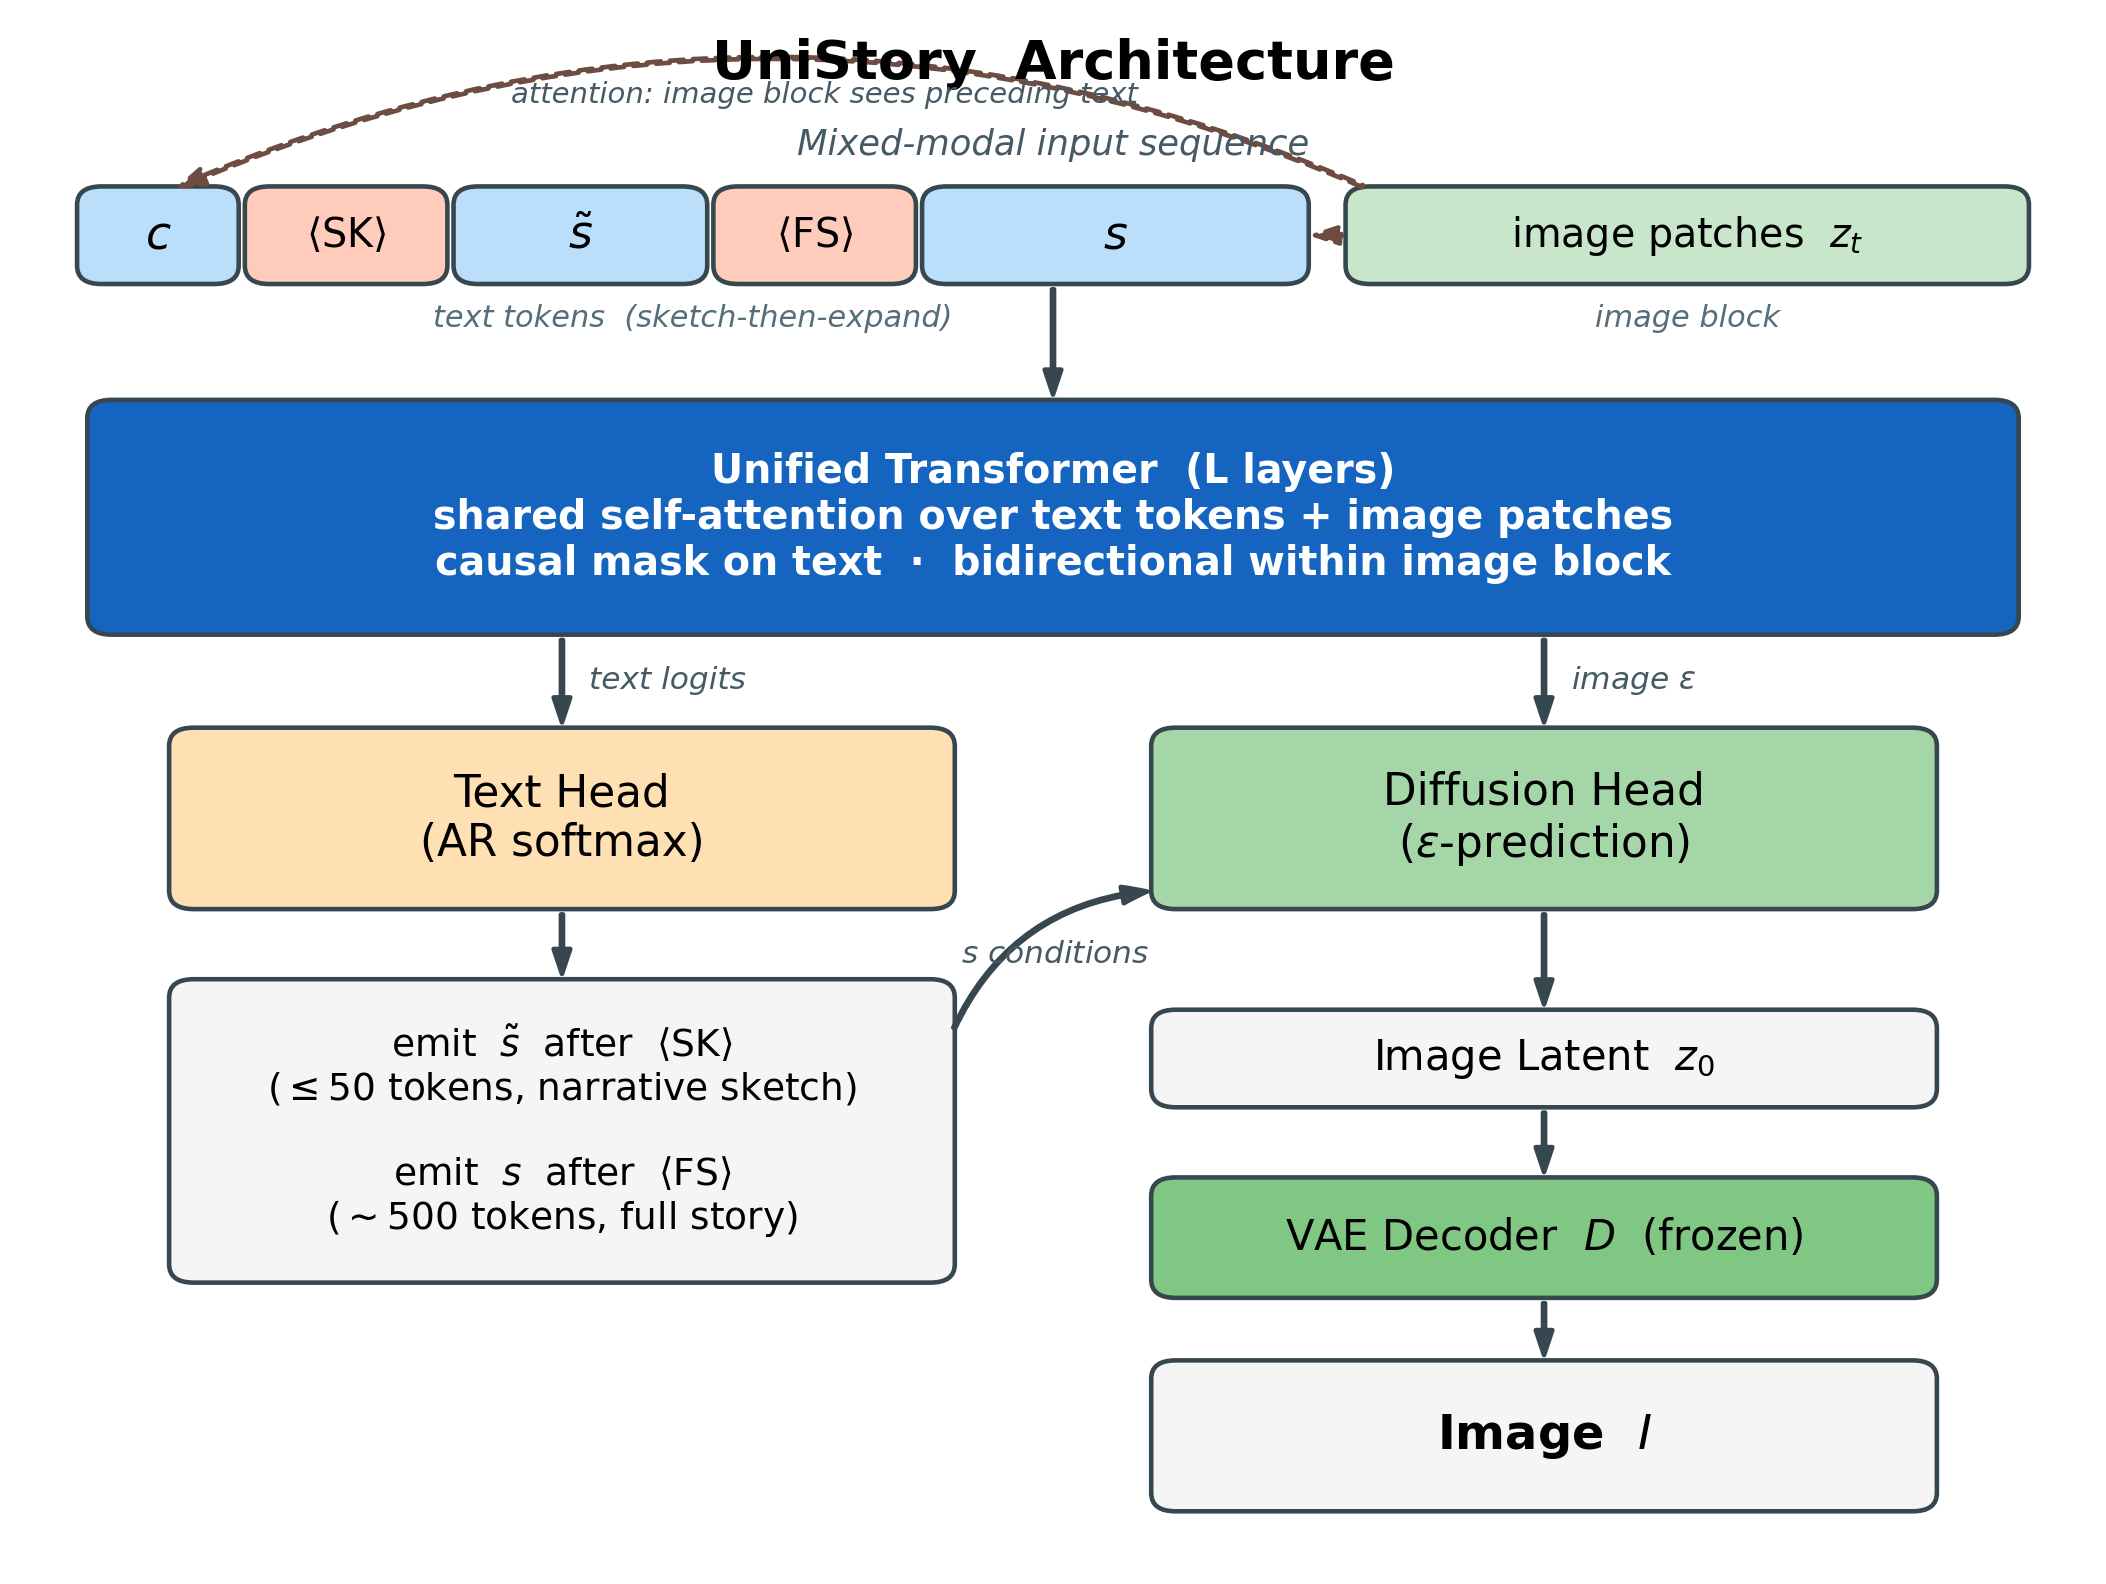
\includegraphics[width=0.48\linewidth]{unistory_architecture.png}
\vspace{-0.8em}
\caption{UniStory interleaves text tokens and image patches in one Transformer. Learned separators $\langle\text{SK}\rangle,\langle\text{FS}\rangle$ split the text side into sketch-then-expand passes; the image block attends to all preceding text, so the diffusion head is conditioned on $c$ and the generated story $s$.}
\label{fig:arch}
\vspace{-1.1em}
\end{figure}

\section{Training Objectives}
\label{sec:loss}

Let $x = (c, s, z_0)$ be a training triple. The \textbf{autoregressive text loss} (chain-rule factorization of the joint probability) is
\begin{equation}
    \mathcal{L}_{\text{LM}}(\theta) \;=\; -\mathbb{E}_{(c,s)}\!\left[\,\sum_{t=1}^{N} \log p_{\theta}\bigl(s_t \mid s_{<t},\, c\bigr)\,\right].
\end{equation}

The \textbf{diffusion loss} on image latents follows DDPM~\citep{ho2020ddpm}, an ELBO on the log-likelihood. With forward process $q(z_t \mid z_0)=\mathcal{N}(z_t; \sqrt{\bar\alpha_t}\, z_0, (1-\bar\alpha_t)\mathbf{I})$, the network $\epsilon_\theta$ predicts the injected noise, conditioned on both the prompt $c$ and the generated story $s$:
\begin{equation}
    \mathcal{L}_{\text{diff}}(\theta) \;=\; \mathbb{E}_{z_0,\,\epsilon,\,t}\!\left[\,\bigl\|\,\epsilon - \epsilon_\theta(z_t, t, c, s)\,\bigr\|_2^2\,\right],\quad \epsilon\sim\mathcal{N}(0,\mathbf{I}),\; t\sim\mathcal{U}\{1,\ldots,T\}.
\end{equation}

A \textbf{cross-modal alignment loss} pulls the generated image toward the story in CLIP space with frozen encoders $\phi_{\text{txt}}, \phi_{\text{img}}$. To keep it differentiable and cheap, we avoid running the full reverse chain and instead use the \emph{$x_0$-prediction shortcut}: at the same sampled $t$ as in $\mathcal{L}_{\text{diff}}$, we reconstruct the clean latent in one step from $\epsilon_\theta$:
\begin{equation}
    \hat{z}_0 \;=\; \frac{z_t - \sqrt{1-\bar\alpha_t}\;\epsilon_\theta(z_t, t, c, s)}{\sqrt{\bar\alpha_t}},\qquad
    \mathcal{L}_{\text{align}}(\theta) \;=\; 1 \;-\; \cos\!\bigl(\phi_{\text{txt}}(s),\; \phi_{\text{img}}(D(\hat{z}_0))\bigr).
\end{equation}

\noindent\textbf{Total objective:}
\begin{equation}
\boxed{\;\mathcal{L}_{\text{UniStory}}(\theta) \;=\; \mathcal{L}_{\text{LM}} \;+\; \lambda_{\text{diff}}\,\mathcal{L}_{\text{diff}} \;+\; \lambda_{\text{align}}\,\mathcal{L}_{\text{align}}\;}
\quad (\lambda_{\text{diff}}{=}1.0,\; \lambda_{\text{align}}{=}0.1).
\end{equation}

\section{Training Strategy and Inference}
\label{sec:train}

\textbf{Training} proceeds in two stages. \emph{Stage 1 (pretraining)}: large-scale image--caption pairs (e.g., LAION-5B) and text-only corpora are used jointly with $\mathcal{L}_{\text{LM}}$ and $\mathcal{L}_{\text{diff}}$; single-modality batches activate only the corresponding term. \emph{Stage 2 (fine-tuning)}: prompt--story pairs $(c, s)$ are harvested from the Reddit WritingPrompts corpus (the top-level comment acts as $s$, the title as $c$); for each pair we synthesize an illustration $I$ by running a frozen pretrained text-to-image teacher (e.g., SDXL) on $s$, and retain triples with $\text{CLIPScore}(s, I)\!\geq\!0.3$ (approximately the top 60\%); $\mathcal{L}_{\text{align}}$ is activated only in this stage. We use AdamW with cosine schedule, classifier-free guidance (CFG) dropout of $c$ and $s$ at 10\% each, and QK-Norm with an auxiliary $z$-loss to stabilize mixed-modal training~\citep{team2024chameleon}.

\textbf{Inference}: (i) sample sketch $\tilde{s}\!\sim\! p_\theta(\cdot\mid c)$; (ii) sample full story $s\!\sim\!p_\theta(\cdot\mid c,\tilde{s})$ with nucleus sampling ($p{=}0.9$); (iii) from $z_T\!\sim\!\mathcal{N}(0,\mathbf{I})$, run $T$ reverse diffusion steps with CFG, $\hat{\epsilon} = (1{+}w)\,\epsilon_\theta(z_t,t,c,s) - w\,\epsilon_\theta(z_t,t,\varnothing)$ where $\varnothing$ denotes dropping both $c$ and $s$ and $w{=}3.0$; decode $I=D(z_0)$.

\textbf{Design justification.} Pure AR image models (e.g., Chameleon) rely on VQ tokenization that caps fidelity; pure diffusion cannot natively generate long coherent text. The hybrid design keeps each paradigm's strength~\citep{zhang2025unified}; conditioning the image on $s$ rather than $c$ captures concrete visual elements (e.g., \emph{``Space Princess Castle''}) that only emerge during story generation.

\setlength{\bibsep}{2pt plus 0.3ex}
{\scriptsize
\bibliographystyle{plainnat}
\bibliography{unistory}
}

\end{document}
